\chapter{Aarsnes-Shor Model}
\label{ch:aarnessshormodel}

\section{Introduction}
The model is developed by Aarsnes and Shor (\referencename~\cite{ref:aarsnes2017a}). It is designed to simulate torsional drill string vibration using a distributed model, wherein the partial difference equations governing the motion are solved using the upwind scheme.   Two versions of the source code are available, one implemented in Matlab and the other in Python.  The Python version is newer and is being written to improve the Matlab version.  Ongoing efforts are focused on enhancing the Python version by incorporating axial motion.

\section{Model Description}
The model simulates torsional vibration of the drill string induced by Coulomb friction and viscous damping which are modeled as distributed source term. The effect of this Coulomb friction becomes prominent as the well inclination increases, therefore this model can be effective in predicting the drill string dysfunctions in high inclined wells. Currently, the model is only applicable for torsional mode simulation but the axial mode will be added soon. The governing equations of torsional motion are solved by finite difference method (FDM) by discretizing the drill string. Assumptions of the model are:
\begin{bulletedlist}
	\item No bit-rock interaction
	\item No lateral and axial motion
	\item The effects of cuttings distribution on the friction is homogeneous
    \item Drill string - well bore friction, dry friction, is modeled as Coulomb friction as a jump.
    \item Both dry and viscous frictions are included in total friction of the system.
\end{bulletedlist}

Two different versions of the codes are available which are written in Matlab and Python. The Matlab ver.\ is more matured and the validation with field data was also conducted \cite{ref:aarsnes2017a}. In comparison, the Python ver.\ is relatively recent version and the axial mode will be added to it. Both codes are based on the same mathematic background and applies finite difference method to solve the torsional vibration of the drill string. However, while Python ver.\ directly solves the governing equation for angular velocity and torque separately, Matlab ver.\ introduces Riemann invariants and combines the torque and angular velocity in the governing equation and solves at once. The comparison between two models are explained in more detail in next section. 

\section{Top Drive Model}
The model contains PI controller on the top drive. Therefore, boundary condition at the top is given by top drive torque and velocity calculated from top drive set point velocity. Torque on top drive are derived as
\begin{equation}\label{AS_err}
  e = w_{sp} - w_{TD}
\end{equation}

\begin{equation}\label{AS_Ie}
  I_e = \int_{0}^{t}e(\xi)d\xi
\end{equation}

\begin{equation}\label{AS_tau_m}
  tau_{td} = K_pe + k_iI_e
\end{equation}
where $w_{sp}$ is set point velocity, $w_{td}$ is top drive velocity, $\tau_{td}$ is top drive torque, $K_p$ and $K_i$ are proportional and integral gain, respectively. $K_p$ and $K_i$ are normally given value from the field. The top drive velocity, $W_{td}$ is then obtained by dynamics
\begin{equation}\label{AS_w_td}
  \frac{\partial w_{td}}{\partial t} = \frac{1}{J_{td}}(\tau_{td} - \tau_0)
\end{equation}
where $J_{td}$ is top drive inertia, $\tau_{0}$ is the torque on top of the drill string. The angular velocity at the top of the drill string is assume to be same as top drive velocity $w_0 = w_{td}$.

\section{Bit Model}
The model assumes the toque on bit to be constant. The Test Cases for this project are off-bottom scenario with not bit-rock contact, therefore, the torque on bit is fixed to zero. In addition, model does not consider weight on bit since current model is only for torsional mode. 

\section{Friction Model}
The total friction including dry and viscous friction, is modeled as Coulomb friction as a jump. The static friction applies when the angular velocity of the drill string is below the given threshold, which is modeled as inclusion. In other words, below the threshold, The total friction is bounded by static friction. On the other hand, when the angular velocity exceeds the threshold, transit to dynamic friction occurs and the total friction will be linear combination of dynamic and viscous friction. More details can be seen from \equationname~\ref{equation_A-S_columnbfriciton}-\ref{equation_A-S_dynamic_fric}. \figurename~\ref{figure_AS_friction} illustrates the friction model for A-S model.
\begin{figure}
  \centering
  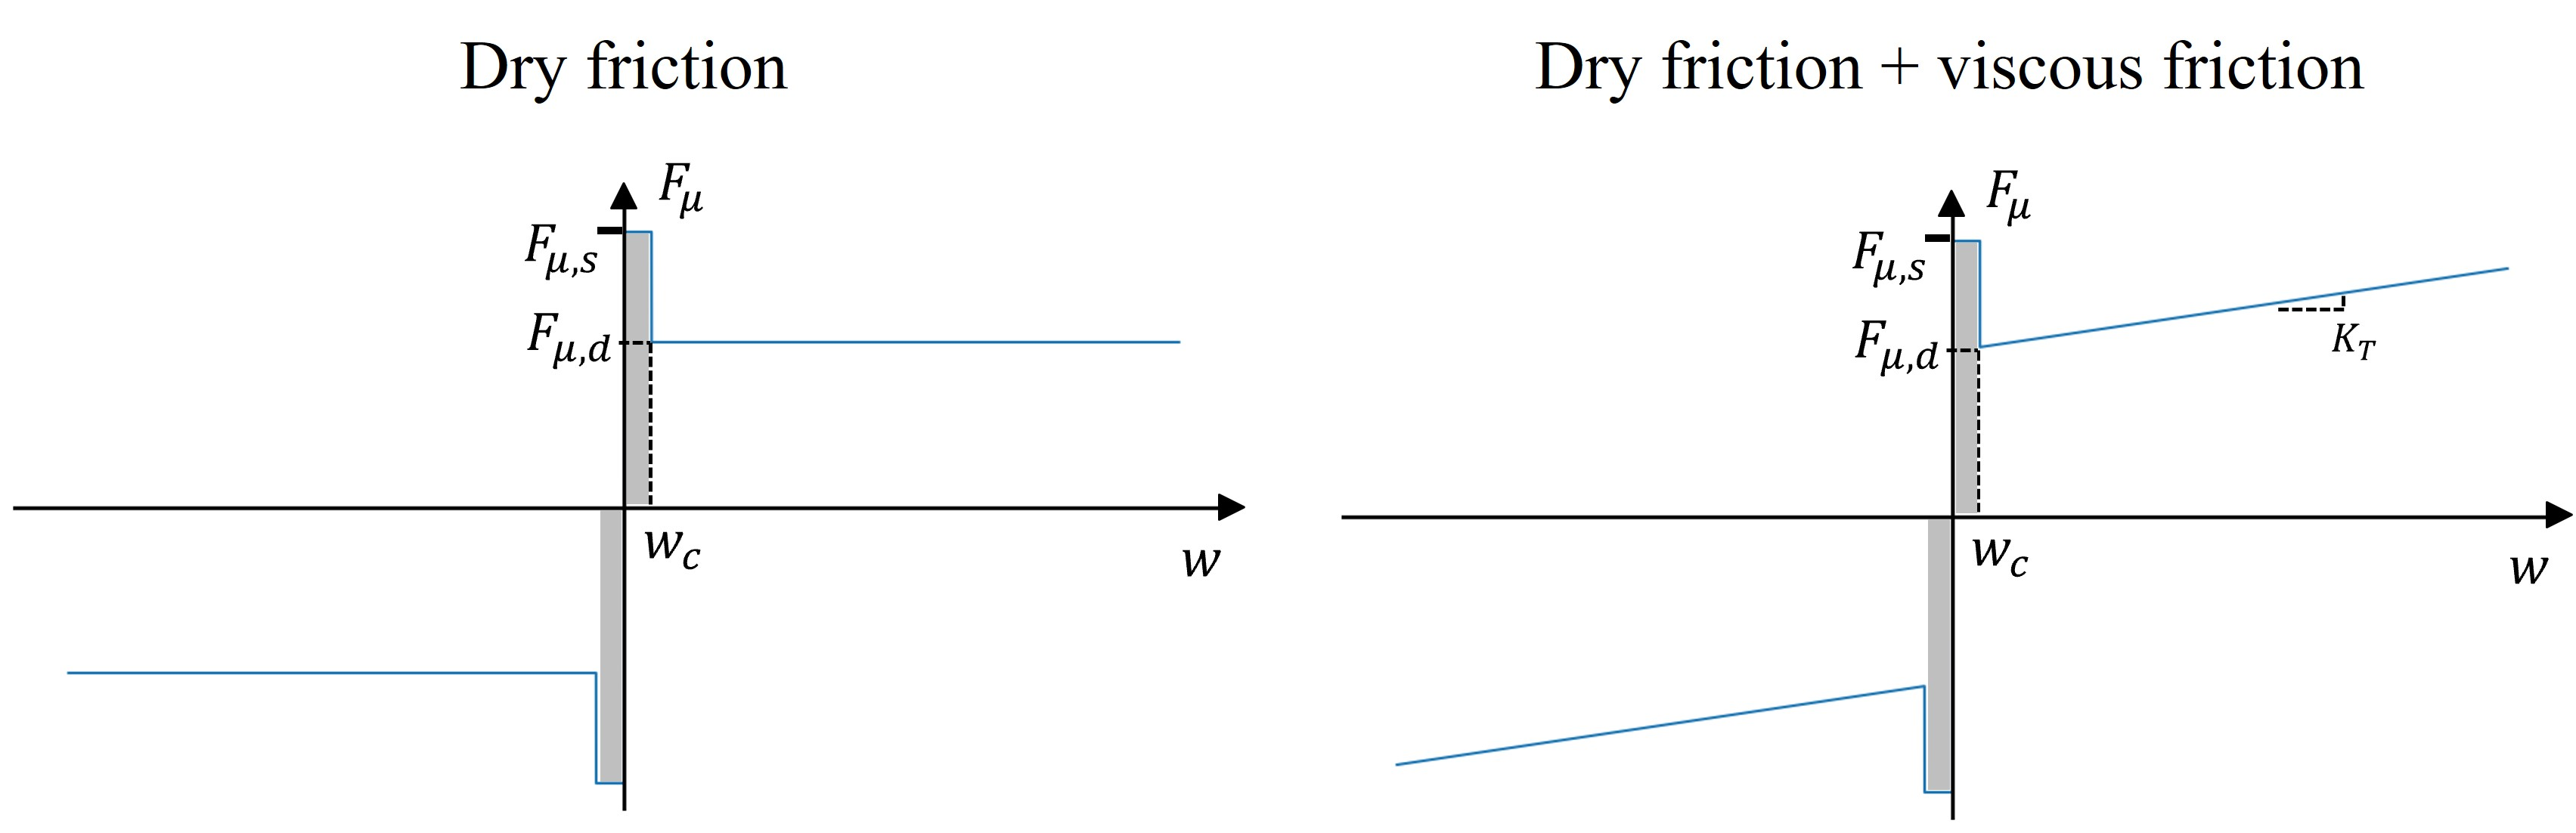
\includegraphics[width=6.5in]{AS_friction}
  \caption[Friction model for A-S model]{Friction model for A-S model. Left and right figures are friction models in A-S model only when dry friction is considered and both dry and viscous friction are included, respectively. Dry friction refers to the friction from drill string and wellbore contact. $F_{\mu, s}$, $F_{\mu, d}$ are static and dynamic friction force, respectively, $k_{T}$ is viscous friction coefficient for torsional motion and $w_{c}$ is critical angular velocity which is the threshold for transition between static and dynamic friction. When the angular velocity is below the critical velocity, the total friction is bounded by static friction.}\label{figure_AS_friction}
\end{figure}

The Coulomb friction $\mathcal{F}(w,x)$ is modeled as an inclusion which is shown in \equationname~\ref{equation_A-S_columnbfriciton}. The parameters for the equations can be seen from \figurename~\ref{figure_AS_equation_schematic}.
\begin{figure}[!hbt]
  \centering
  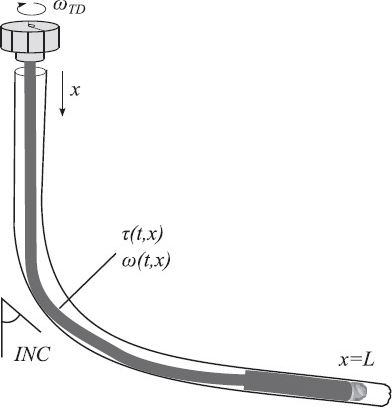
\includegraphics[width=2.5in]{AS_parameters}
  \caption[Schematic of distributed drill string in deviated well]{Schematic of distributed drill string in deviated well and indication of parameters used in the equations \cite{ref:aarsnes2017a}.}\label{figure_AS_equation_schematic}
\end{figure}
\begin{equation}\label{equation_A-S_columnbfriciton}
  \begin{cases}
     \mathcal{F}(w,x) = F_{\mu,d}(x), & \mbox{if } w>w_c \\
     \mathcal{F}(w,x) \in [-F_{\mu,s}(x), F_{\mu,s}(x)], & \mbox{if } |w|<w_c \ \\
     \mathcal{F}(w,x) = -F_{\mu,d}(x), & \mbox{if } w < -w_c.
  \end{cases}
\end{equation}
where $w_c$ is the critical angular velocity for Coulomb friction transition from static to dynamic, $F_{\mu,d}$ and $F_{\mu,s}$ are dynamic and static Coulomb torque, respectively. For condition $|w|<w_c$, $\mathcal{F}(w,x)$ takes the boundary values $\pm F_{\mu,s}(x)$.

Static friction $F_{\mu,s}$ is calculated from normal force, $F_N$, along the drill string which is obtained as
\begin{equation}\label{equation_AS_normal_force}
  F_n(x) = gA(x)(\rho-\rho_{mud})sin\theta
\end{equation}
where A(x) is the cross sectional area at location x,  $\rho, \rho_{mud}$ are material and mud density, respectively.
Then the static friction is calculated as
\begin{equation}\label{equation_A-S_static_fric}
  F_{\mu,s}(x,\mu_s) = \mu_sr_o(x)F_N(x)
\end{equation}
where $r_o(x)$ is the outer radius of the drill string at location x. 
On the other hand, the dynamic friction is calculated as a pre-established ratio of static friction. Therefore the dynamic friction is expressed as
\begin{equation}\label{equation_A-S_dynamic_fric}
  F_{\mu,d}(x,\mu_s) = fRat F_{\mu,s}(x,\mu_s)
\end{equation}
\section{Mathematical Background}\label{SubSec_AS_mathematicalbackground}
\subsection{Governing Equations}
The model is based on the equations of angular motion, here named wave equation, which are
\begin{equation}\label{AS-motion}
  J\rho\frac{\partial w(t,x)}{\partial t} + \frac{\partial \tau (t,x)}{\partial x} = S(w,x) 
\end{equation}
\begin{equation}\label{AS-motion1}
 \frac{\partial\tau(t,x)}{\partial t} + JG\frac{\partial w(t,x)}{\partial x} = 0 
\end{equation}
where J is polar moment of inertia and $\rho$ is material density, $w(t,x)$ is angular velocity, $\tau(t,x)$ is torque and S is the source term which can be represented as
\begin{equation}\label{AS-sourceterm}
  S(w,x) = -k_t \rho J w(t,x) - \mathcal{F}(w,x)
\end{equation}
where $k_t$ is damping constant which is viscous shear stresses from drilling mud and cuttings bed and $\mathcal{F}(w,x)$ is Coulomb friction between the drill string and the borehole that is derived from \equationname~\ref{equation_A-S_columnbfriciton}-\ref{equation_A-S_dynamic_fric}.

\subsection{Numerical Implementation of Matlab ver.}
\subsubsection{Riemann Invariants}
The partial governing equations \equationname~\ref{AS-motion} and \ref{AS-sourceterm} are transformed into their Riemann invariants solved by first order upwind scheme. The Riemann invariants are defined as
\begin{equation}\label{AS-Riemann}
  \alpha = w + \frac{c_t}{JG}\tau, \quad \beta=w-\frac{c_t}{JG}\tau
\end{equation}
where $c_t = \sqrt{\frac{\rho}{J}}$ is the velocity of the torsional wave. It can be noticed that angular velocity and torque can be obtained from the relationships
\begin{equation}\label{equation_Riemann_relation1}
  \frac{\alpha + \beta}{2} = w
\end{equation}
\begin{equation}\label{equation_Riemann_relation2}
  J \rho \frac{\alpha + \beta}{2c_t} = \tau
\end{equation}
and the variable $\alpha$, $\beta$ satisfies the PDE system 
\begin{equation}\label{AS-Riemann_alpha}
  \frac{\partial \alpha}{\partial t} + c_t\frac{\partial \alpha}{\partial x} = -\mathcal{S}
\end{equation}
\begin{equation}\label{AS-Riemann_beta}
  \frac{\partial \beta}{\partial t} - c_t\frac{\partial \beta}{\partial x} = -\mathcal{S}
\end{equation}
Therefore, angular velocity w and torque $\tau$ can be obtained by solving $\alpha$ and $\beta$.
The source term $\mathcal{S}$ is
\begin{equation}\label{AS-source}
  \mathcal{S} = \frac{S}{J \rho} j= k_t(\alpha + \beta) + \frac{1}{J \rho} \mathcal{F}
\end{equation}
where $k_t$ is damping coefficient and $\mathcal{F}$ is Coulomb friction defined in \equationname~\ref{equation_A-S_columnbfriciton}. 
\subsubsection{Boundary Condition}
The boundary conditions are given as:
\begin{equation}\label{AS-BC}
  w_{p,top} = w_{td} \quad \tau_{c,bottom} = \tau_{bit}
\end{equation}
where subscript p, c represents drill pipe and drill collar. In this project, $\tau_{bit}$ is assumed to be 0 with the off-bottom scenario. 
Additionally, the conditions at the drill pipe - drill collar interface are imposed:
\begin{equation}\label{AS-interface}
  w_{p,interface} = w_{c,interface}, \quad \tau_{p,interface} = \tau_{c,interface}
\end{equation}
The boundary and interface condition is then expressed for $\alpha$ and $\beta$. \figurename~\ref{AS_discretizeDS} illustrates the schematic view of the discredited drill string with boundary conditions and interface conditions in terms of Riemann invariants.

\equationname~\ref{AS-BC} can be re-written from the relationship from \equationname~\ref{equation_Riemann_relation1} and \ref{equation_Riemann_relation2} as
\begin{equation}\label{AS-riemannBC}
  \alpha_{p,top} = -\beta_{p,top} + 2*w_{te}, \quad \beta_{c,bottom} = \alpha_{c,bottom} - 2\tau_{bit} \frac{c_t}{J_c G_c}
\end{equation}
Also, \equationname~\ref{AS-interface} can be re-written as
\begin{equation}\label{AS-riemanninterface}
\begin{split}
    & \beta_{p,bottom} = \frac{1}{1+\overline{Z}}\left(\alpha_{p,bottom}(1-\overline{Z}) + 2\overline{Z}\beta_{c,top} \right) \\
    & \alpha_{c,top} = \frac{1}{1+\overline{Z}}\left(2*\alpha_{p,bottom} - \beta_{c,top}(1-\overline{Z})\right)
\end{split}
\end{equation}
where $\overline{Z}$ is the relative magnitude of the impedance that is
\begin{equation}\label{AS_Zbar}
  \overline{Z} = \left[\frac{c_t}{JG}\right]_{p,bottom} / \left[\frac{c_t}{JG}\right]_{c,top}
\end{equation}
\begin{figure}[!hbt]
  \centering
  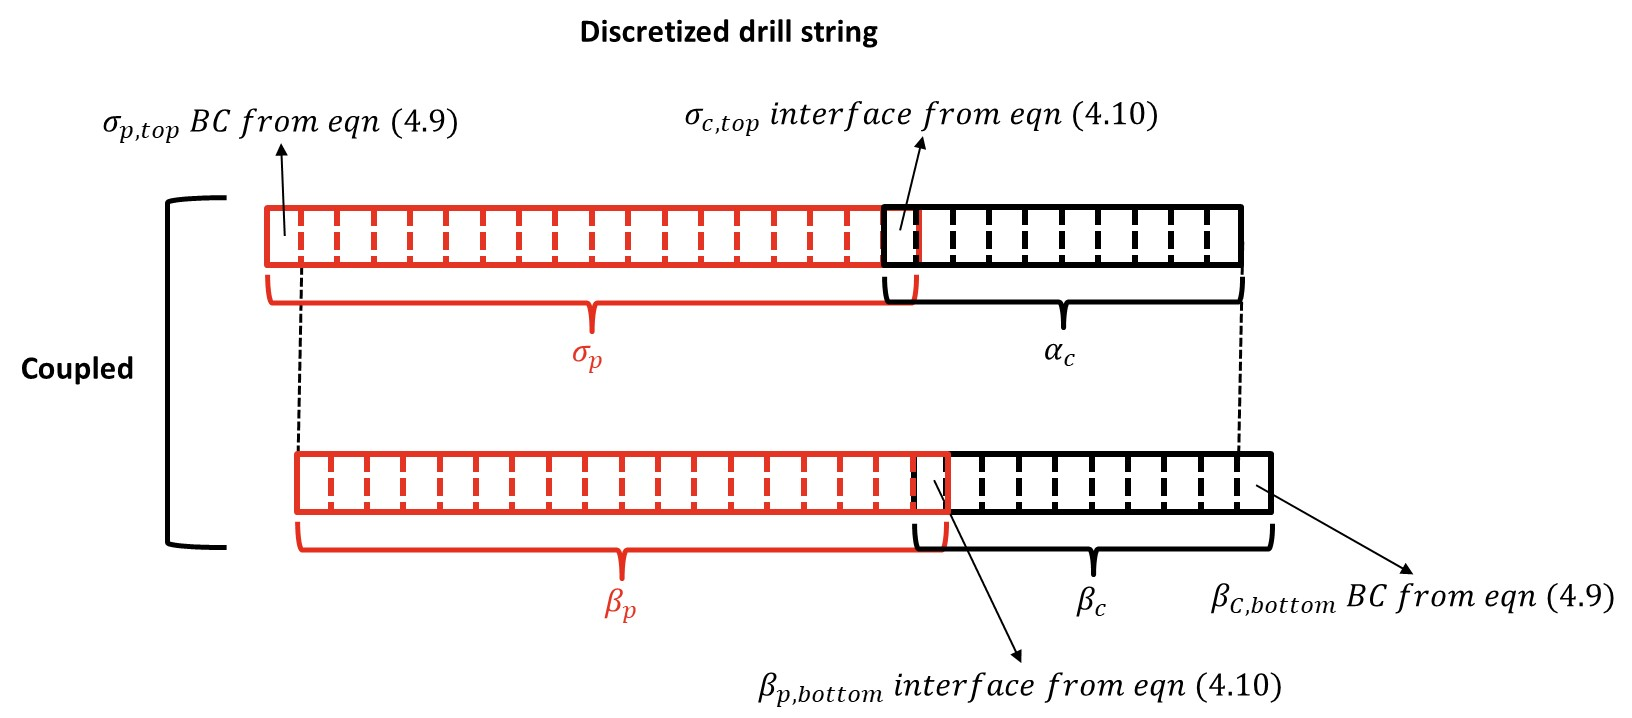
\includegraphics[width=6in]{AS_discretizedDS}
  \caption[Schematic of discretized drill string and boundary conditions]{Schematic of discretized drill string, boundary conditions and interface conditions based on Riemann invariants $\alpha$ and $\beta$.}\label{AS_discretizeDS}
\end{figure}

\subsubsection{Forward Scheme}
The PDE is solved from upwind scheme. First, the Coulomb friction is updated by \equationname~\ref{AS-upwind}, which is driven by rearranging \equationname{}s~\ref{AS-Riemann_alpha}-\ref{AS-source}.
\begin{equation}\label{AS-upwind}
  \mathcal{F}_{j}^k = \frac{\rho J}{2 \Delta t}\left(a_j^k - c_t \frac{\Delta t}{\Delta x}(a_j^k - a_{j-1}^k) + \beta_j^k + c_t \frac{\Delta t}{\Delta x}(\beta_{j+t}^k-\beta_j^k) + \Delta t k_t (\alpha_j^k + \beta_j^k)\right)
\end{equation}
which is for sell size $\Delta x$ and time step $\Delta t$, at cell j and time step k.
Then, $\mathcal{F}_{j}^k$ is limited by \equationname~\ref{equation_A-S_columnbfriciton} and \ref{equation_A-S_dynamic_fric}, which can be expressed in Riemann invariants as:
\begin{equation}\label{equation_A-S_columnbfriciton_Riemann}
\mathcal{F}_{j}^k =
  \begin{cases}
      max(min(\mathcal{F}_{j}^k,{F_C}_j^k),-F_{C,j}^k) , & \mbox{if } \frac{|\alpha_j^k + \beta_j^k|}{2} \le w_c \\
      sign(\frac{|\alpha_j^k + \beta_j^k|}{2}){F_C}_j^k fRat; , & \mbox{if } \frac{|\alpha_j^k + \beta_j^k|}{2} \ge w_c \\
  \end{cases}
\end{equation}
where ${F_C}_j^k$ is the static friction calculated at cell j and time step k. Finally, Riemann invariants are updated iteratively by upwind scheme as:
\begin{equation}\label{equation_upwind_alpha}
  \alpha_j^{k+1} = \alpha_j^{k} - c_t \frac{\Delta t}{\Delta x}(\alpha_j^k - \alpha_{j-1}^k) - \Delta t k_t (\alpha_j^k + \beta_j^k) - \mathcal{F}_j^k
\end{equation}
\begin{equation}\label{equation_upwind_beta}
  \beta_j^{k+1} = \beta_j^{k} - c_t \frac{\Delta t}{\Delta x}(\beta_{j+1}^k - \beta_{j}^k) - \Delta t k_t (\alpha_j^k + \beta_j^k) - \mathcal{F}_j^k
\end{equation}
\subsection{Numerical Implementation of Python ver.}
The Python ver.\ directly solves the \equationname~\ref{AS-motion} and \ref{AS-motion1} by FDM (forward-time-centered-space) rather than introducing Riemann invariants like in the Matlab ver.\ The angular velocity and torque are updated iteratively from the algorithm below. The parameters in the algorithm are listed in \tablename~\ref{AS_inptut_params}. 
\begin{table}[!hbt]
\centering
\begin{tabularx}{\linewidth-0.75in}{|c|c|L|}
\hline
\tablecolumnheadervlinesone{Parameter} & \tablecolumnheadervlinestwo{Units} & \tablecolumnheadervlinestwo{Notes} \\                                                              
\hline
Simulation length & s & Total simulation time \\                                                                                                    
\hline
$w_c$ & rad/s & Cut-off angular velocity (static, dynamic transition)\\                                                              
\hline
$\mu_s$ & -& Static friction factor\\
\hline
$\mu_k$ & - & Kinetic friction factor \\ 
\hline
$K_t$ &- & Inertial torsional damping \\                                                  
\hline
$K_s$ &- & Viscous damping coefficient \\                                                   
\hline
$\rho$ & $lbf/ft_3$ & Drill string density \\                                                       
\hline
G & $lbf/ft^2$ & Shear modulus   \\                                                                                                                     
\hline
$K_p$ & $lb$-$ft$ & P-gain of top drive (PI controller) \\
\hline
$K_i$ & $lb$-$ft/s$ &I-gain of top drive (PI controller)\\ 
\hline
$J_{TD}$ & $lb$-$ft^2$ & Top drive inertia \\
\hline
Ramp speed & $RPM$/s & Ramp speed of top drive\\
\hline
\end{tabularx}
\caption[Input parameters of Aarsnes-Shor model (Python ver.)]{Input parameters of Aarsnes-Shor model. well trajectory, top drive set velocity and bit constant are the additional parameters which are not included in this table.}\label{AS_inptut_params}
%\end{tabular}
\end{table}

\newcommand{\codecomment}[1]{\hfill #1}
\pushinitialcodeindent{0in}
\begin{code}[\codenumbering]{}
\codeitemnonumber \pseudocodefor{} i = 1 simulation length/$\Delta t$
	\stepcodelevel{}
	\codeitemnonumber nstep = freq/$\Delta t$ \codecomment{Freq=frequency of removing the noise}
	\codeitemnonumber \pseudocodefor{} {j=1:nstep}
		\stepcodelevel{}
	    \codeitemnonumber 1. Set the top drive set point torque and angular velocity
	    \codeitemnonumber $w_{sp}(t+1)=w_{sp}(t)\pm ramp \cdot dt$
	    \codeitemnonumber $e=w_{sp}(t+1)-w_{td}(t), \quad I=e \cdot dt$
	    \codeitemnonumber $\tau_{td}(t+1) \gets \tau_{td}(t) + (k_e e + k_i I) \cdot dt$
	    \codeitemnonumber $w_{td}(t+1) \gets w_{td}(t) + (\tau_{td}(t+1)-\tau_{top}(t))/J_{td} \cdot dt$
	    \codeitemnonumber 2. Bit rotation
	    \codeitemnonumber $\tau_{bit}(t+1) \gets bitconstant \cdot w_{bottom}(t)$
	    \codeitemnonumber $w_{bit}(t+1) \gets w_{bottom}(t)$
	    \codeitemnonumber 3. Update top drive torque 
	    \codeitemnonumber $\tau_{TD}(t+1) \gets \tau_{TD}(t+1)-J_{TD}(w_{TD}(t+1)-w_{TD}(t))/dt$
	    \codeitemnonumber 4. Calculate source term
	    \codeitemnonumber $fric \gets \mu_k \cot f_n \cdot r_o$ \codecomment{Coulomb friction}
	    \codeitemnonumber $Iner \gets k_t \cdot \rho \cdot J \cdot (w(t)-w(t-1))$ \codecomment{Inertia damping}
	    \codeitemnonumber $vis \gets k_s \cdot w(t)$ \codecomment{Viscous damping}
	    \codeitemnonumber $S \gets (fric+iner+vis)/dx$
	    \codeitemnonumber 5. Update the torque and angular velocity \codecomment{eqn.\ref{AS-motion} and \ref{AS-motion1}}
	    \codeitemnonumber $\tau(t+1) \gets \tau(t) - JG \cdot dl/dt (w_n(t)-w_{(n-1)}(t))$ \codecomment{n is discretized number}
	    \codeitemnonumber $w(t+1) \gets w(t) 2 \cdot dt/(J \cdot \rho)\left[(\tau_n(t)-\tau_{n-2}(t))/(2*dx)+S\right]$
	    \prevcodelevel{}
	\codeitemnonumber \pseudocodedonefor{}
	\codeitemnonumber $\overline{w} \gets \overline{w} \cdot Kernel$ \codecomment{remove high frequency noise}
	\codeitemnonumber $\overline{\tau} \gets \overline{\tau} \cdot Kernel$
	\prevcodelevel{}
\codeitemnonumber \pseudocodedonefor{}
\end{code}
\popinitialcodeindent{}
\section{Findings and Code Modifications}
Some findings are reported in this section and the tests were conducted based on Test Case 1 scenario. Please refer to \chaptername~\ref{ch:testcases} for detail description and input parameters for each Test Case.

\subsection{Effect of PI Controller}
The A-S model contains PI controller on top drive for more realistic simulation, however; the results were sensitive to input parameters which are $k_p, k_i, J_{TD}$ and ramp speed. Therefore, it was difficult to compare between different models when the exact value of these parameters were not provided. \figurename~\ref{figure_topdrive_sensitivity} illustrates the comparison between Matlab ver.\ and Python ver.\ when same top drive related parameters used 
(\tablename~\ref{table_topdrivesensitivity_input}). Please note that the model was run with same input parameters with different units (Matlab ver: Metric unit, Python ver: Imperial unit). 

\begin{testcasetable}
$k_p$ & $38e^3 \; lbf\cdot ft/s $ & $28e^3\; Nm/s$ & P-gain \\                                                  
\hline
$k_i$ & $100e^3 \; lbf\cdot ft$ & $74e^3\; Nm$  & I-gain \\                                                  
\hline
$J_{TD}$ & $2900 \; lb\cdot ft^2 $ & $ 68818 \; kgm^2$ & Top drive inertia\\                                                       
\hline
\end{tabularx}
\caption[Top drive related parameters for comparison]{Top drive related parameters for comparison between A-S model Matlab and Python versions.}\label{table_topdrivesensitivity_input}
\end{testcasetable}

\begin{figure}
  \centering
  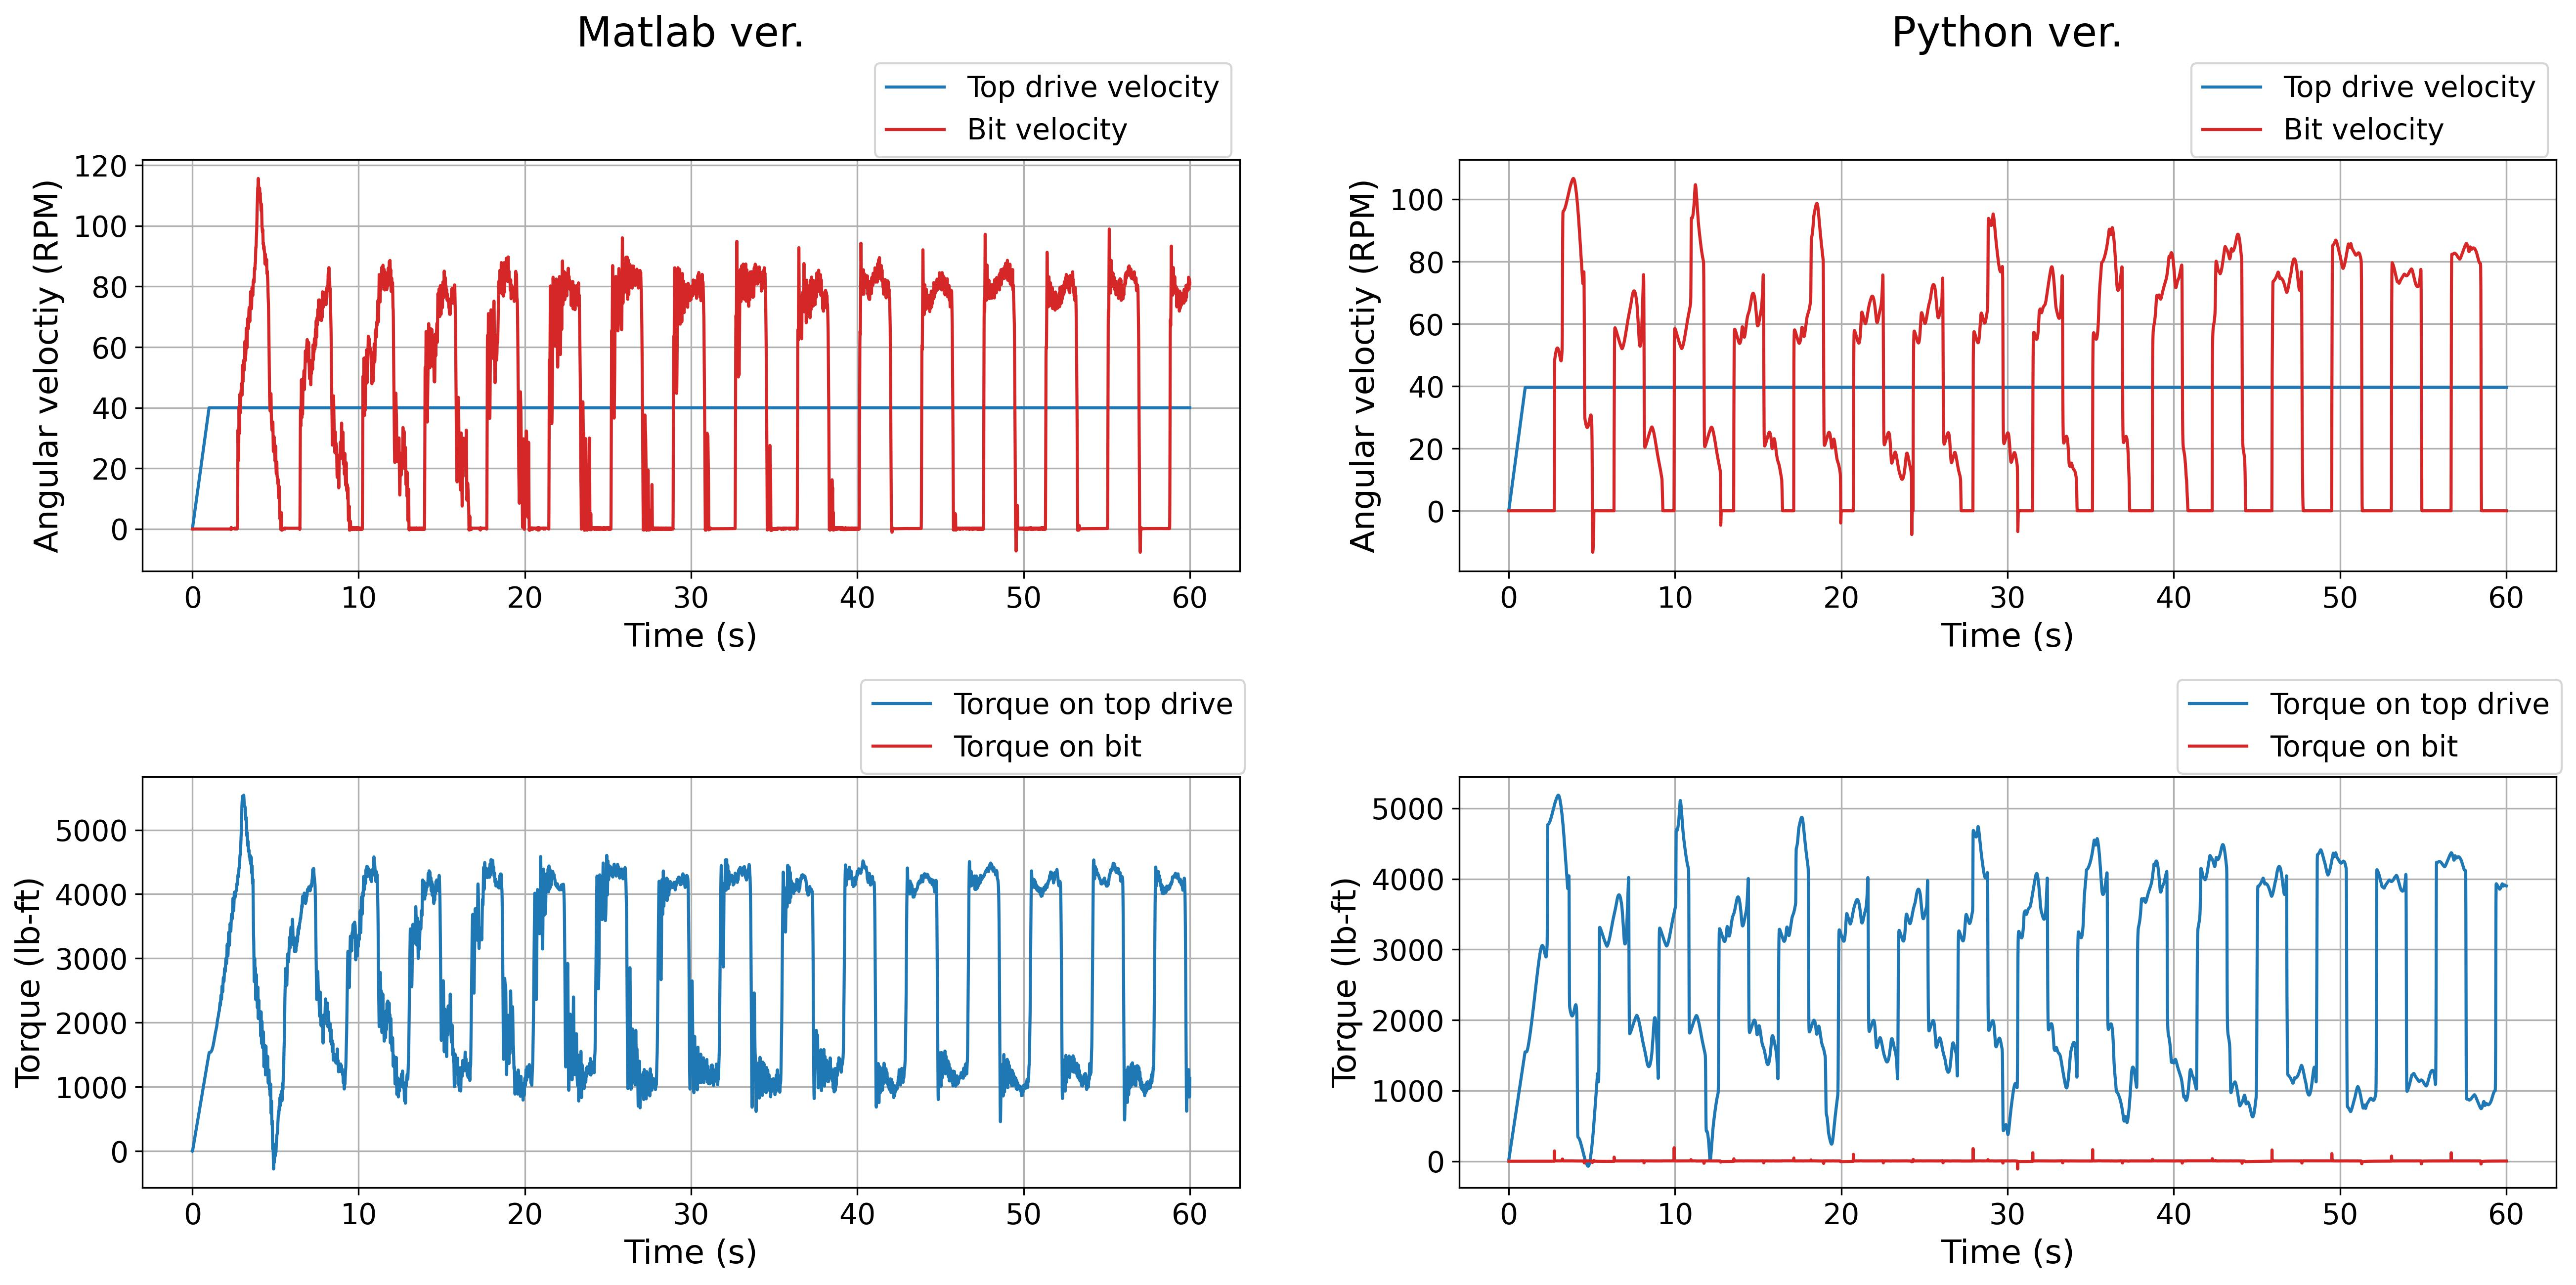
\includegraphics[width=6.5in]{PI_comp}
  \caption[Comparison of drill string response to same top drive parameters]{Comparison of top drive and bit responses with same top drive parameters between Matlab ver.\ and Python ver.\ First and second columns are results from Matlab ver. and from Python ver., respectively}\label{figure_topdrive_sensitivity}
\end{figure}
The results implies that, for the further study, exact input parameters are required or the PI controller should be removed. Therefore, the codes were modified and top drive was removed from the system assuming the fixed velocity at the top of the drill string. Moreover, The modified code enables reducing the parameters of the model for more simple comparison between different models. The flowchart of PI controller removal is shown in \figurename~\ref{figure_Topdriveremove_math}. 

\begin{figure}
  \centering
  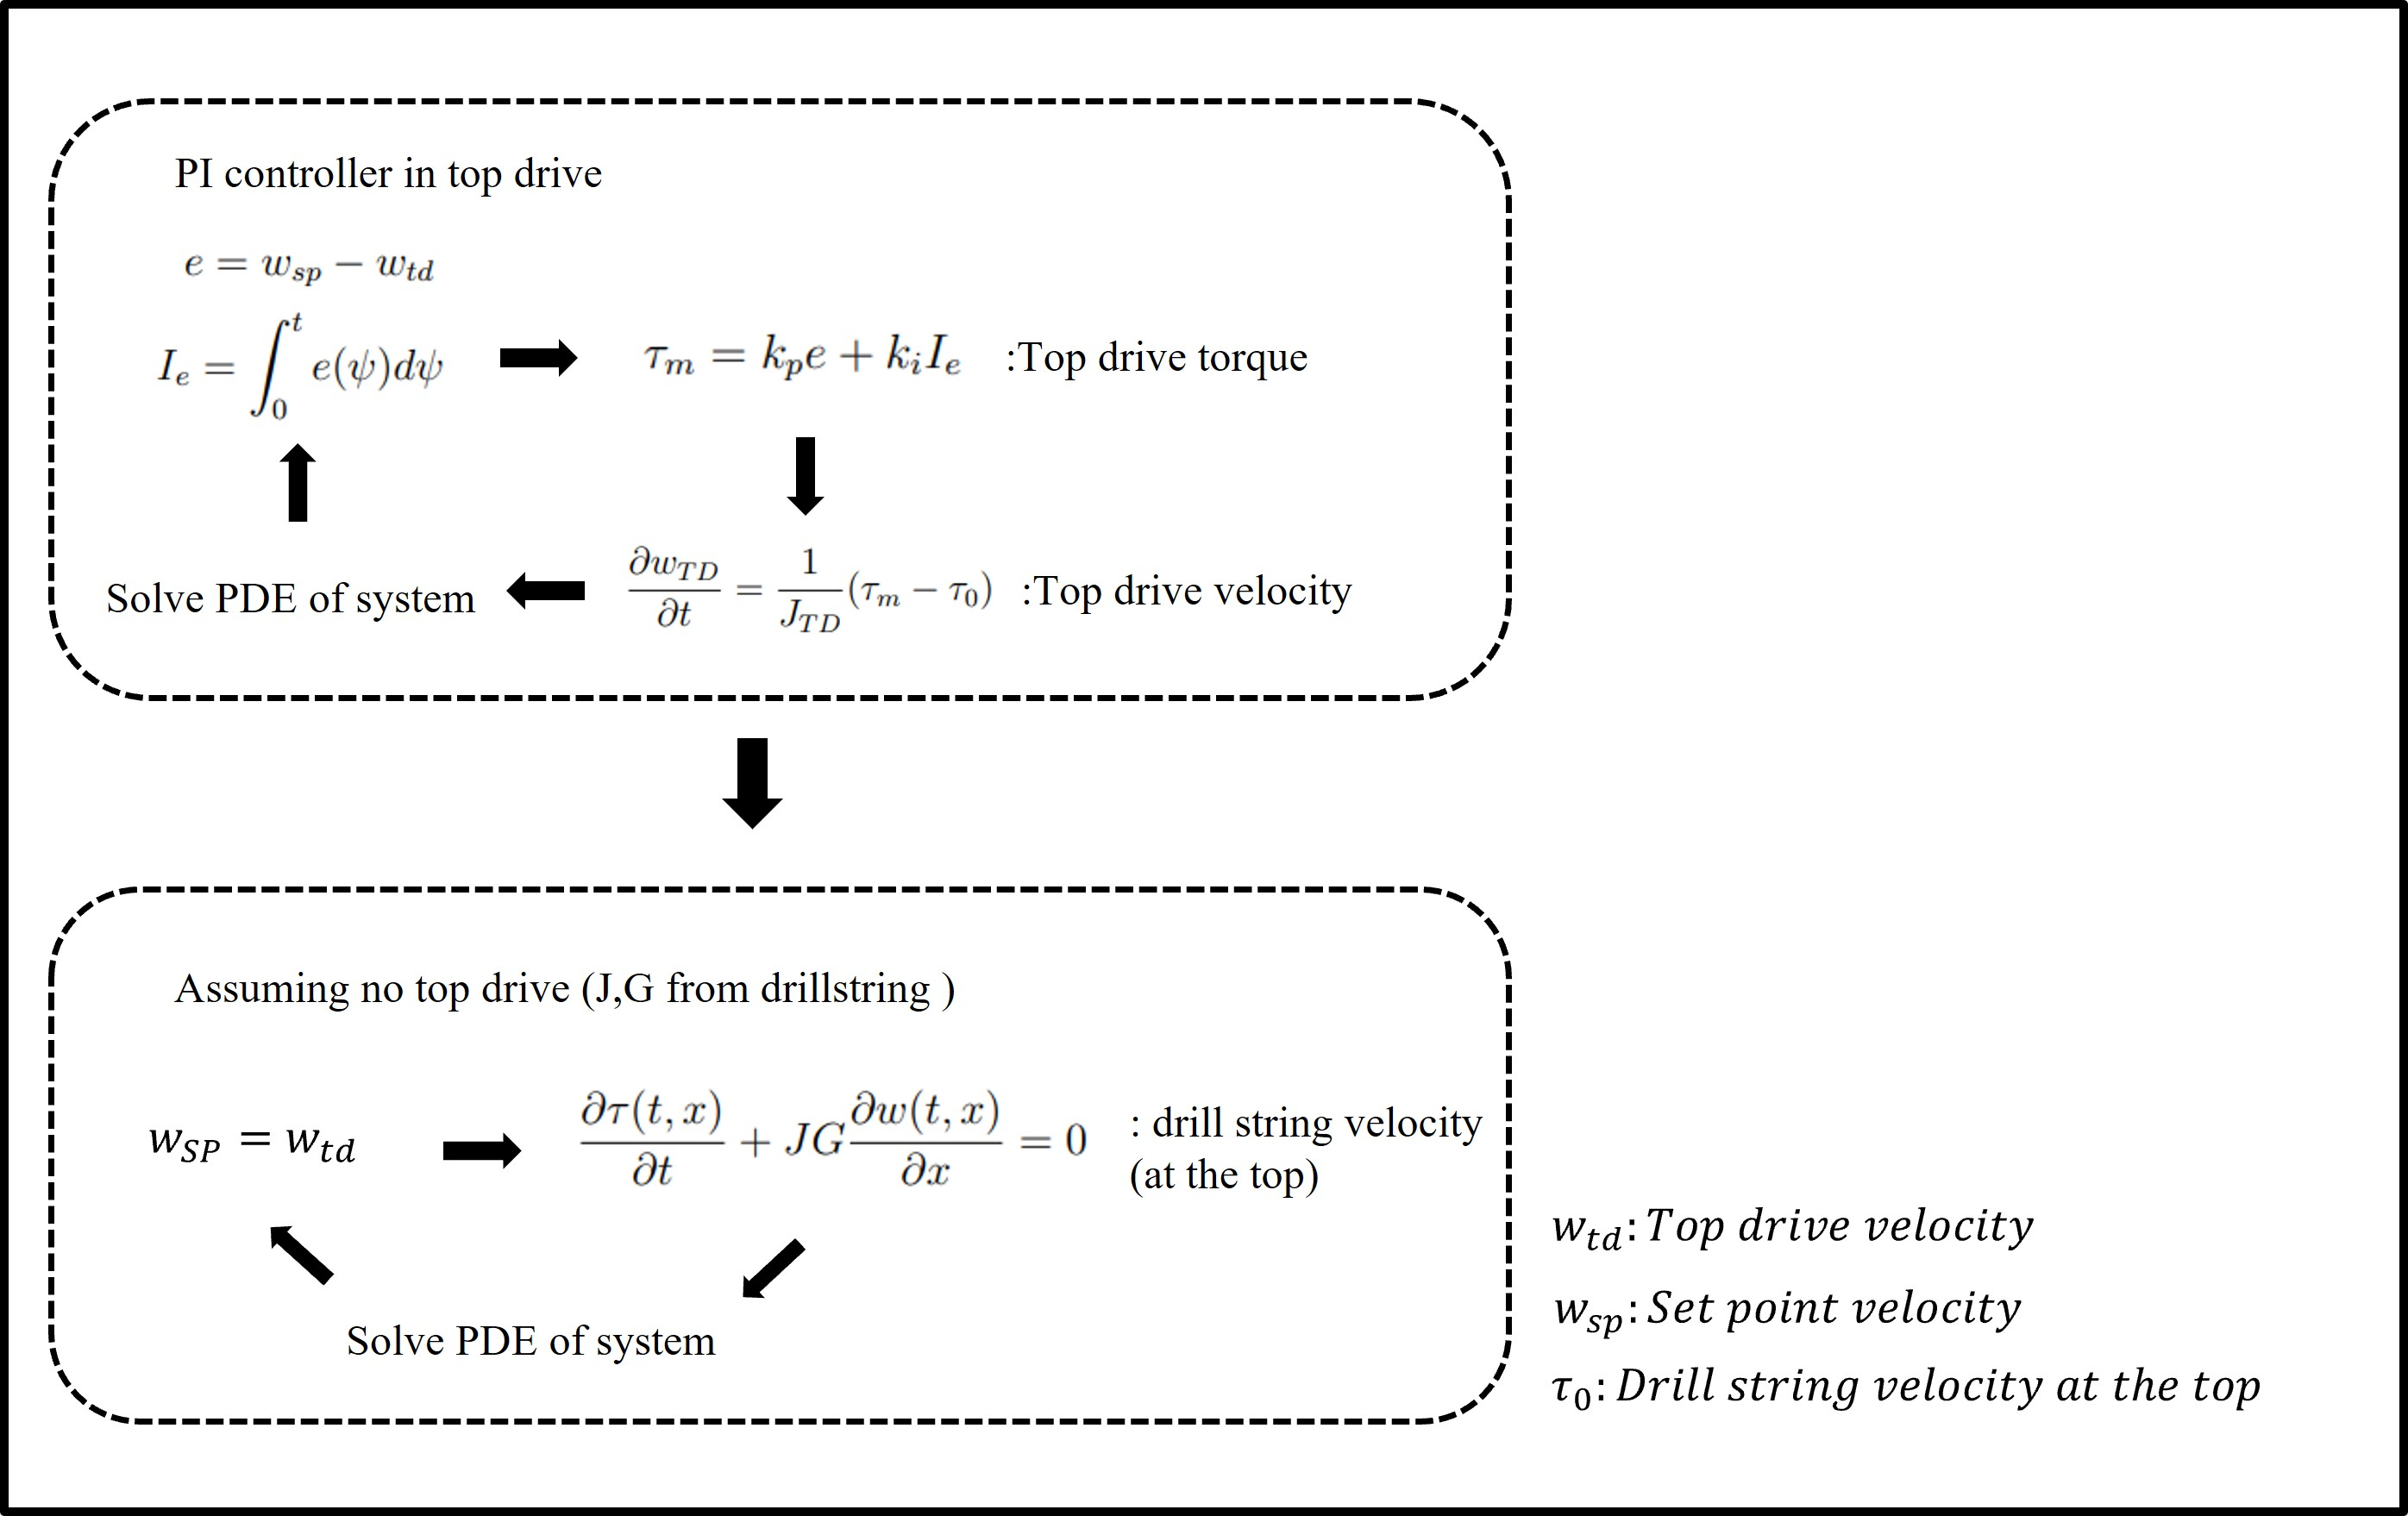
\includegraphics[width=6in]{Topdriveremove_math}
  \caption[Flow chart of top drive elimination]{Flow chart of top drive elimination. The modification of the model assumes only drill string in the model and it rotates with given (fixed) velocity at the top of the drill string.}\label{figure_Topdriveremove_math}
\end{figure}

The comparison of angular velocity and torque of top drive and bit between when the top drive is existed and removed are depicted in \figurename~\ref{figure_topdriveremove_Matlab} and \ref{figure_topdriveremove} for Matlab and Python ver, respectively. In the modified code, top drive velocity and torque will refer that of top of the drill string. The original and modified code showed almost the same behavior except during the very first stage when the top drive set point velocity increased from 0 to 40 $RPM$ (from 0 to 1 second). The spikes can be seen when the top drive includes PI controller. Additionally, the decaying of the vibration amplitude was observed when the simulation was run with PI controller, which can be clearly seen in the Matlab ver.\ This is due to the damping effect from the PI controller while controlling the top drive velocity and it eventually converges the vibration.

In summary, removing the PI controller enables us to obtain a model with reduced parameters and eliminates the damping effect from the PI controller. This simplification of the model results in a advantage in model comparison, particularly for this project. However, if the PI controller is available in the rig, simulation with PI controller can provide more accurate results for field application.
\begin{figure}[!hbt]
  \centering
  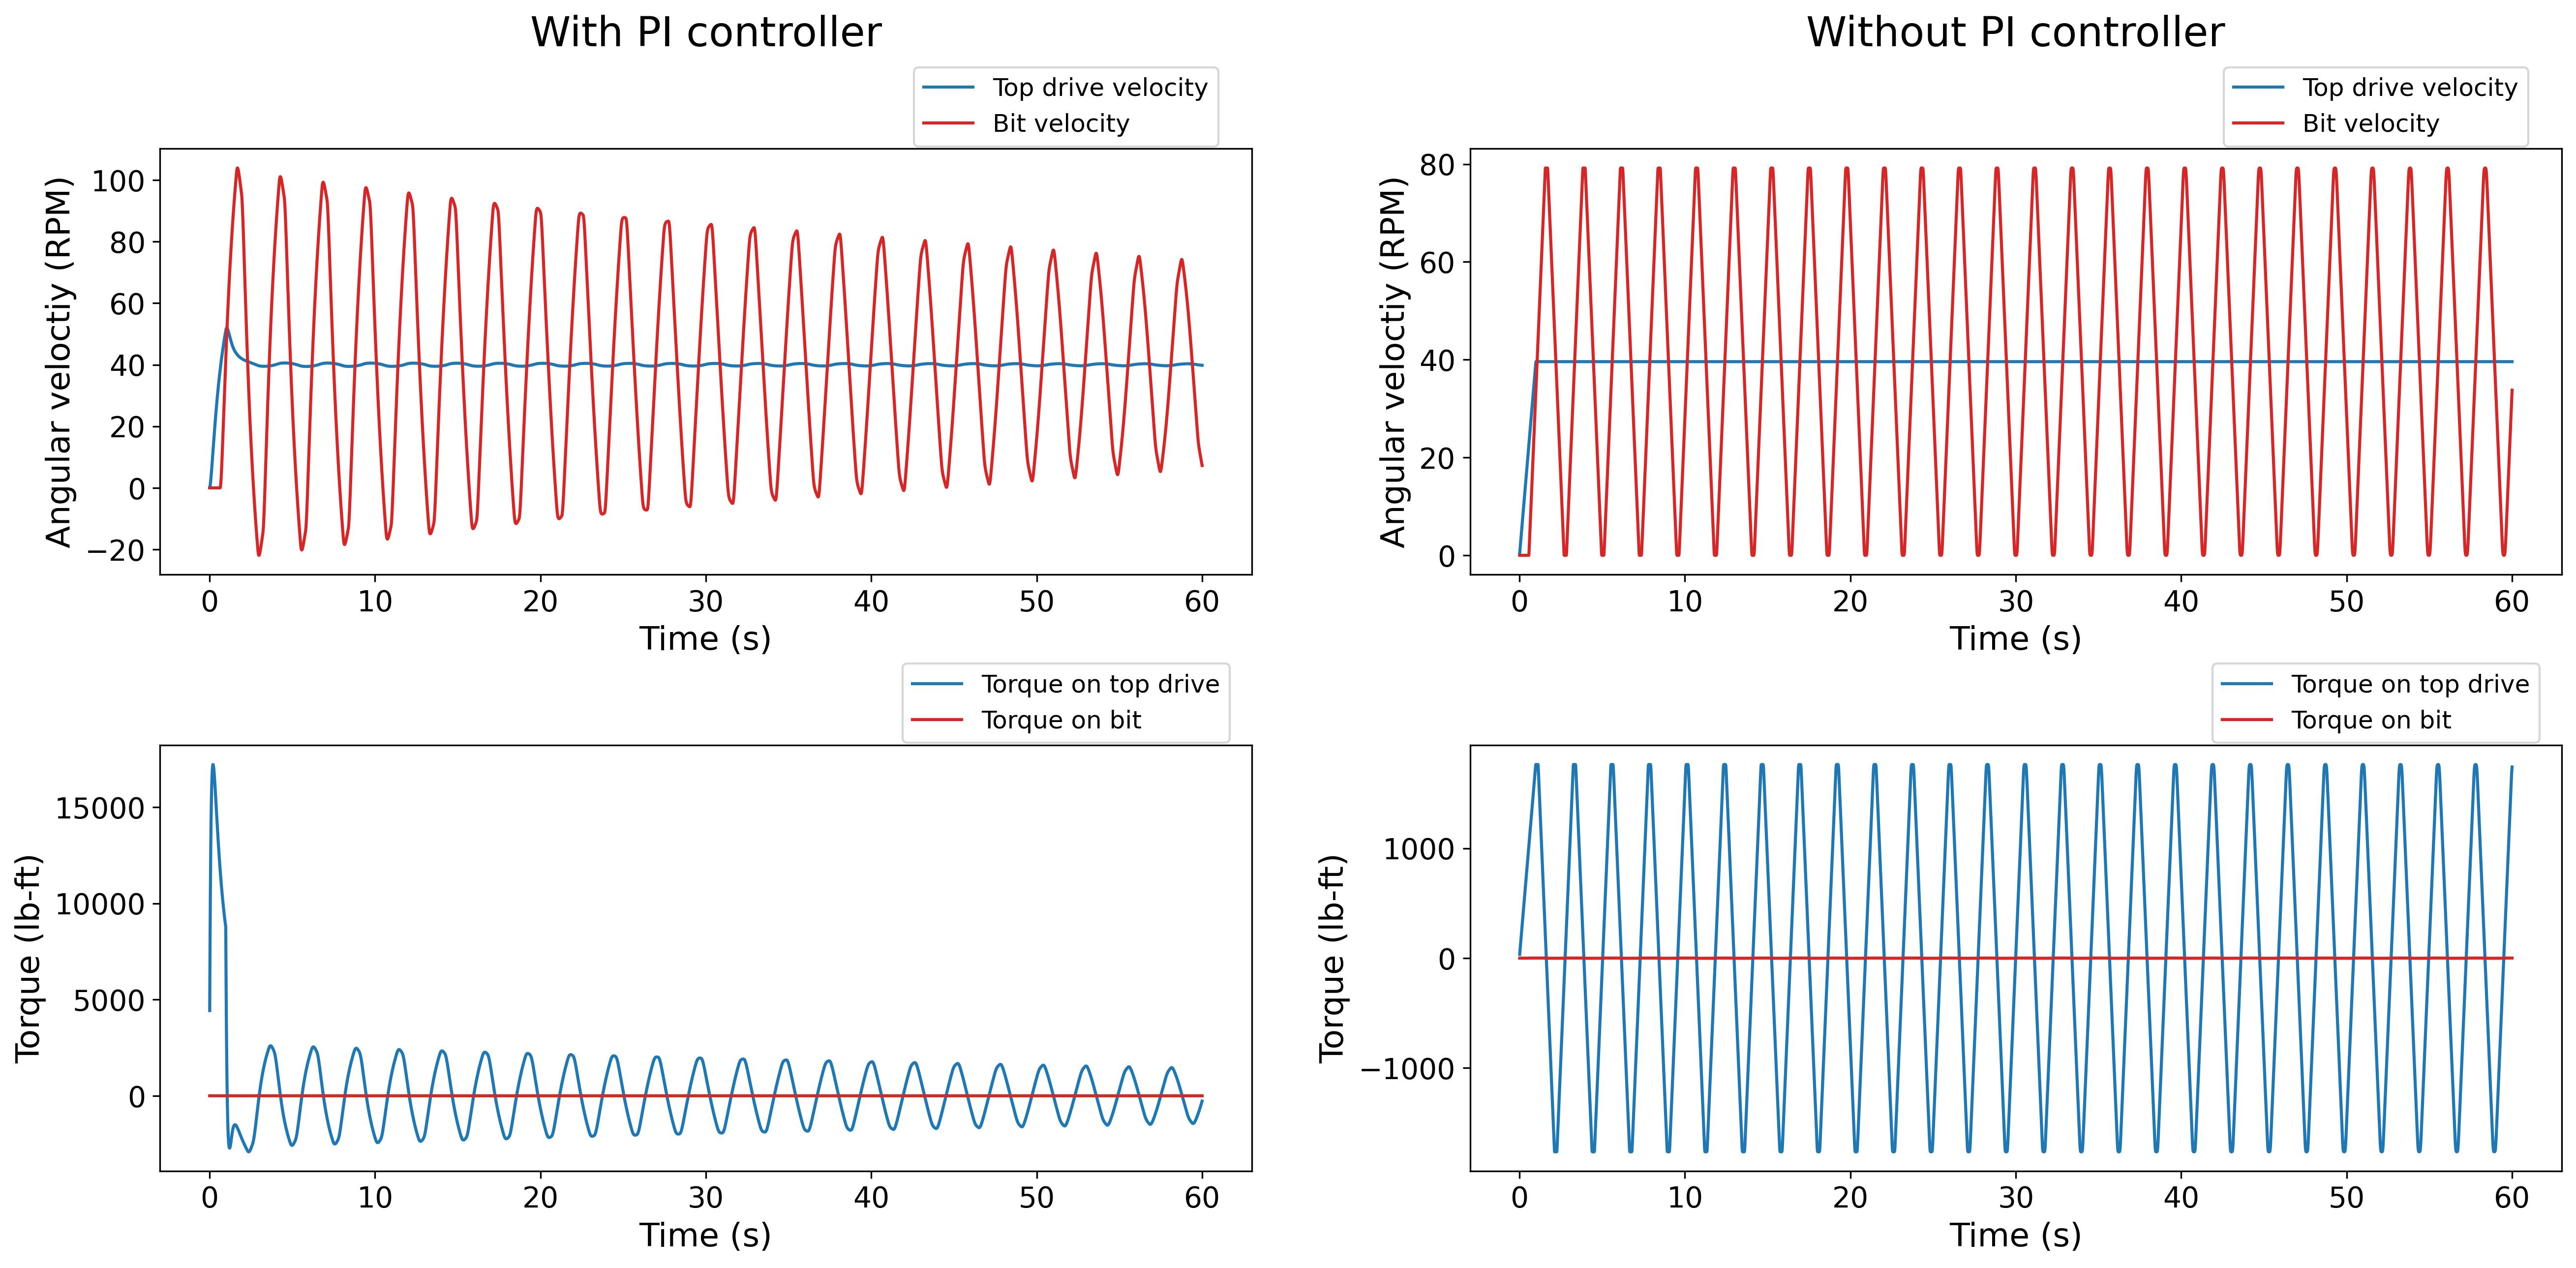
\includegraphics[width=6.5in]{PI_matlab}
  \caption[Comparison between with and without top drive: Matlab ver]{Comparison of the angular velocity and torque of the top drive and bit when top drive with and without PI controller in top drive in A-S model, Matlab ver.\ First and second columns represent the results with and without PI controller.}\label{figure_topdriveremove_Matlab}
\end{figure}

\begin{figure}[!hbt]
  \centering
  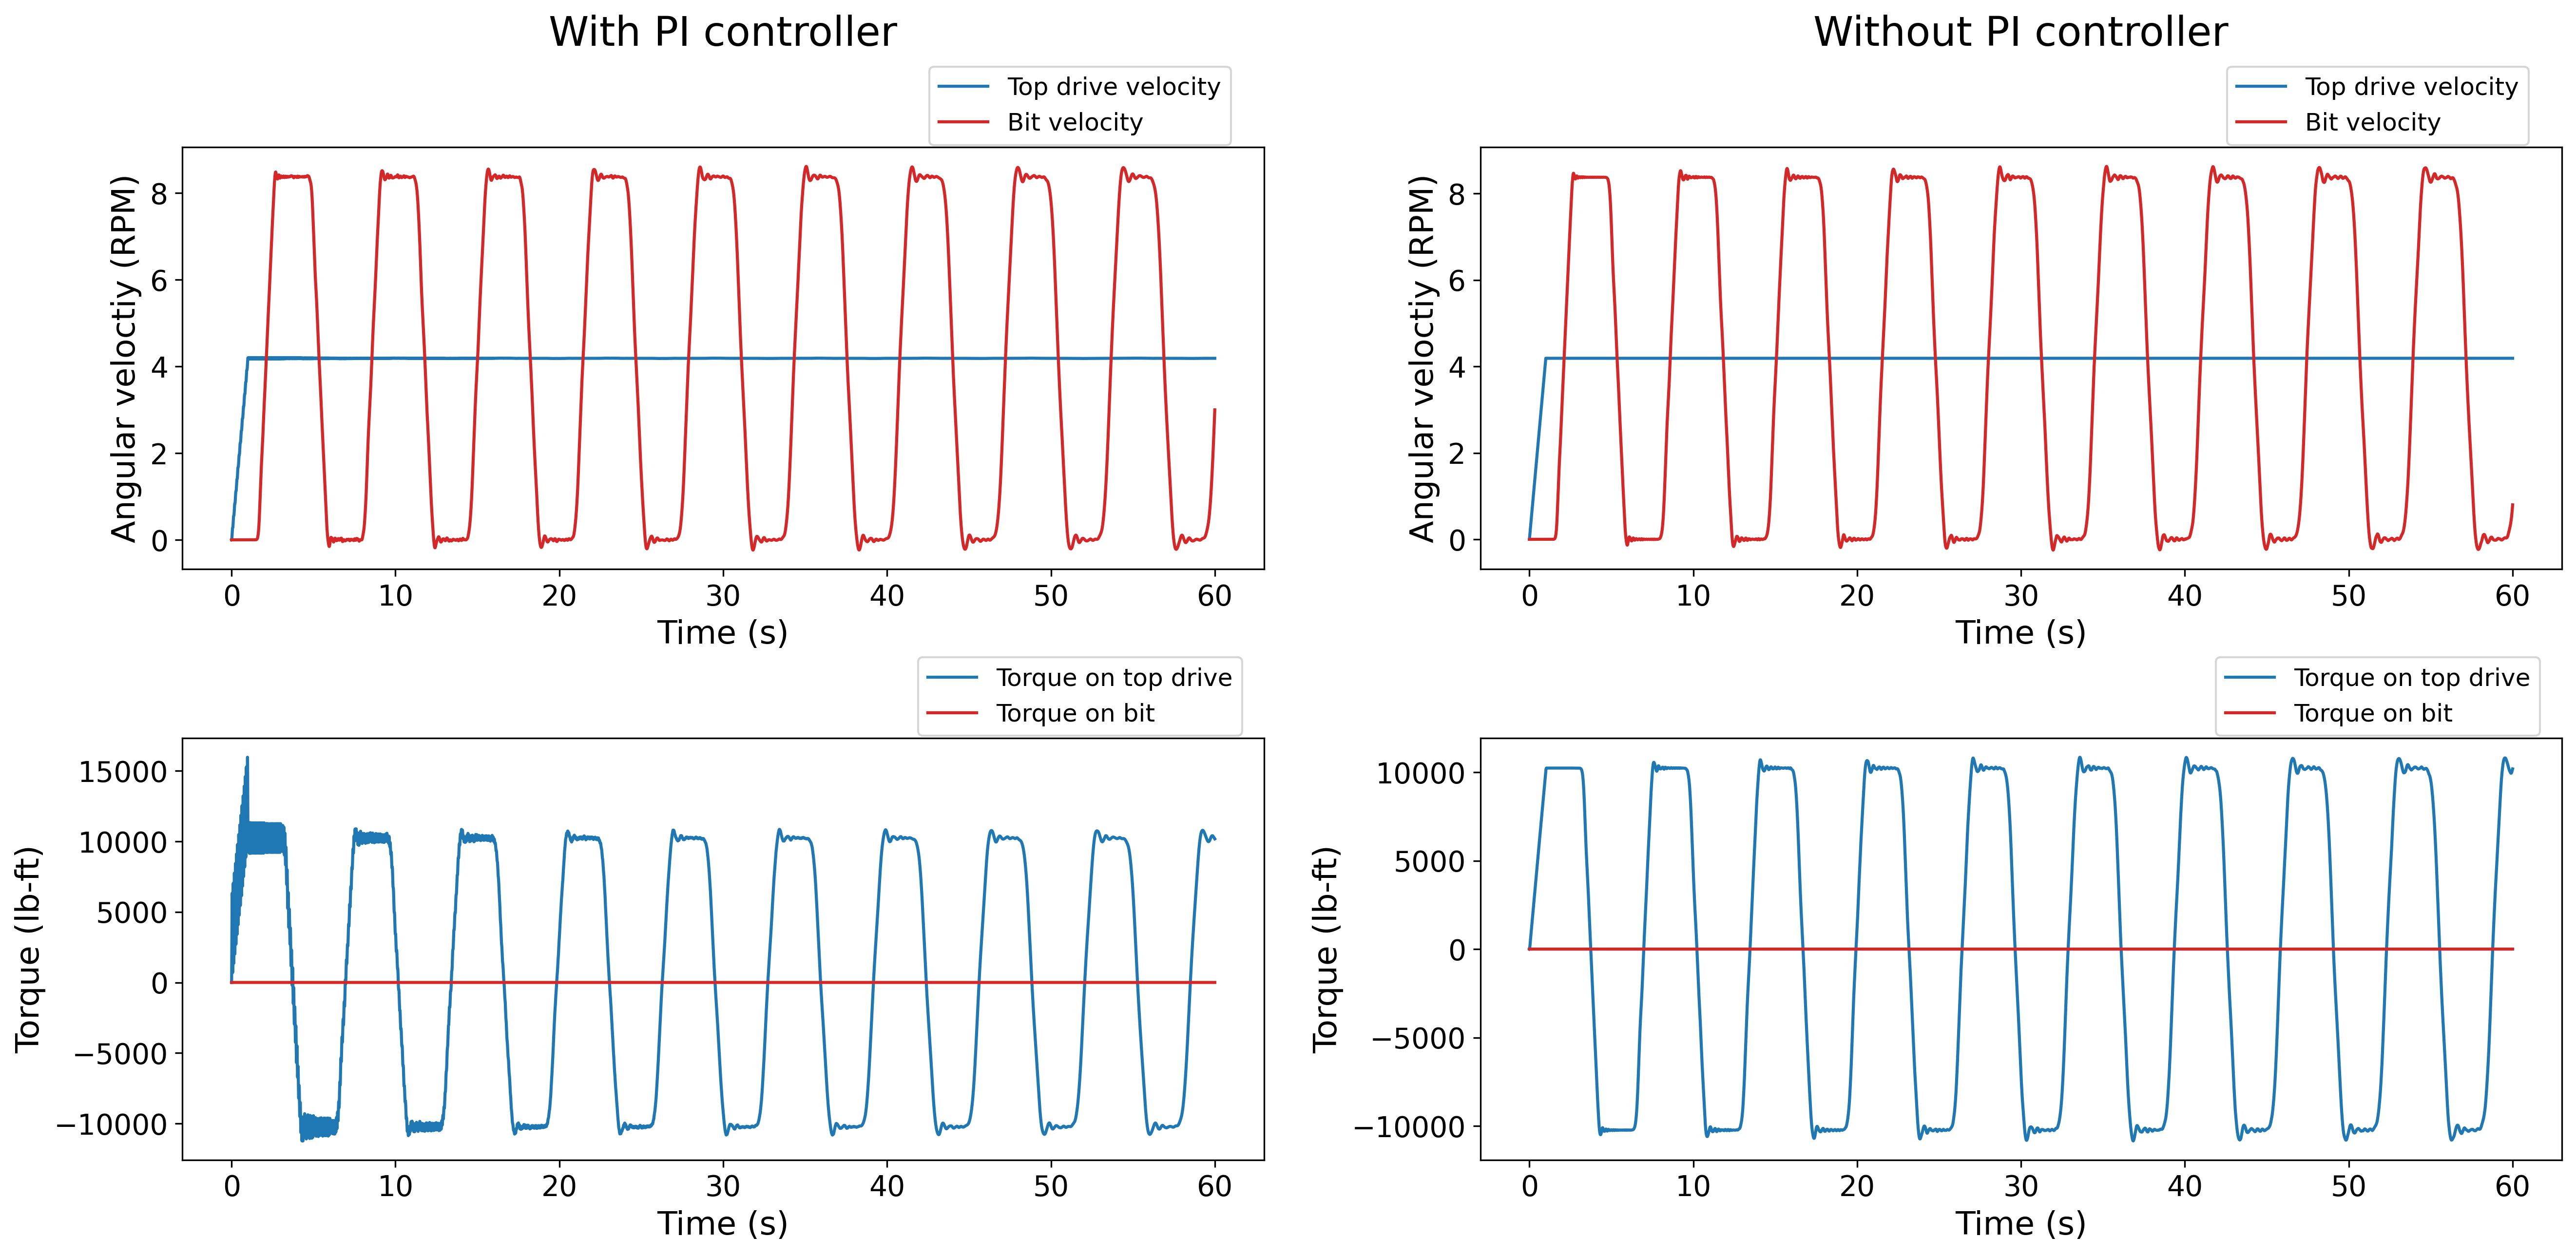
\includegraphics[width=6.5in]{PI_python}
  \caption[Comparison between with and without top drive: Python ver]{Comparison of the angular velocity and torque of the top drive and bit when top drive with and without PI controller in top drive in A-S model, Python ver.\ First and second columns represent the results with and without PI controller.}\label{figure_topdriveremove}
\end{figure}

\subsection{Comparison Between Matlab and Python Ver.}
The model of Matlab ver.\ and Python ver.\ were compared before conducting the tests to validate the model. The comparison was conducted with Test Case 1 scenario. The Python ver.\ showed different patterns of bit and top drive compared to Matlab ver.\ there was a period where bit angular velocity and top drive torque maintained at maximum value for about 2 seconds. The comparison between the Matlab and Python ver.\ can be seen in \figurename~\ref{figure_Test1_comp_chASmodel} with results from ExxonMobil model for reference. The Python ver.\ showed different results, which assumed to be caused by the difference in wave travel velocity along the drill string, which is proportional to $\sqrt{\rho/J}$. By decreasing the density to $1/4$ of the default input (490.50 $lb/ft^3$ $\rightarrow$ 122.65 $lb/ft^3$), Python ver.\, similar result to Matlab ver.\ and ExxonMobil ver.\ was obtained. (\figurename~\ref{figure_Python_reducedDensity}). The modification of the Python code has not been made yet. Therefore, only Matlab ver.\ AS model and ExxonMobil model will be used for the final results and discussions in \chaptername~\ref{ch:results}.

\begin{figure}[!hbt]
  \centering
  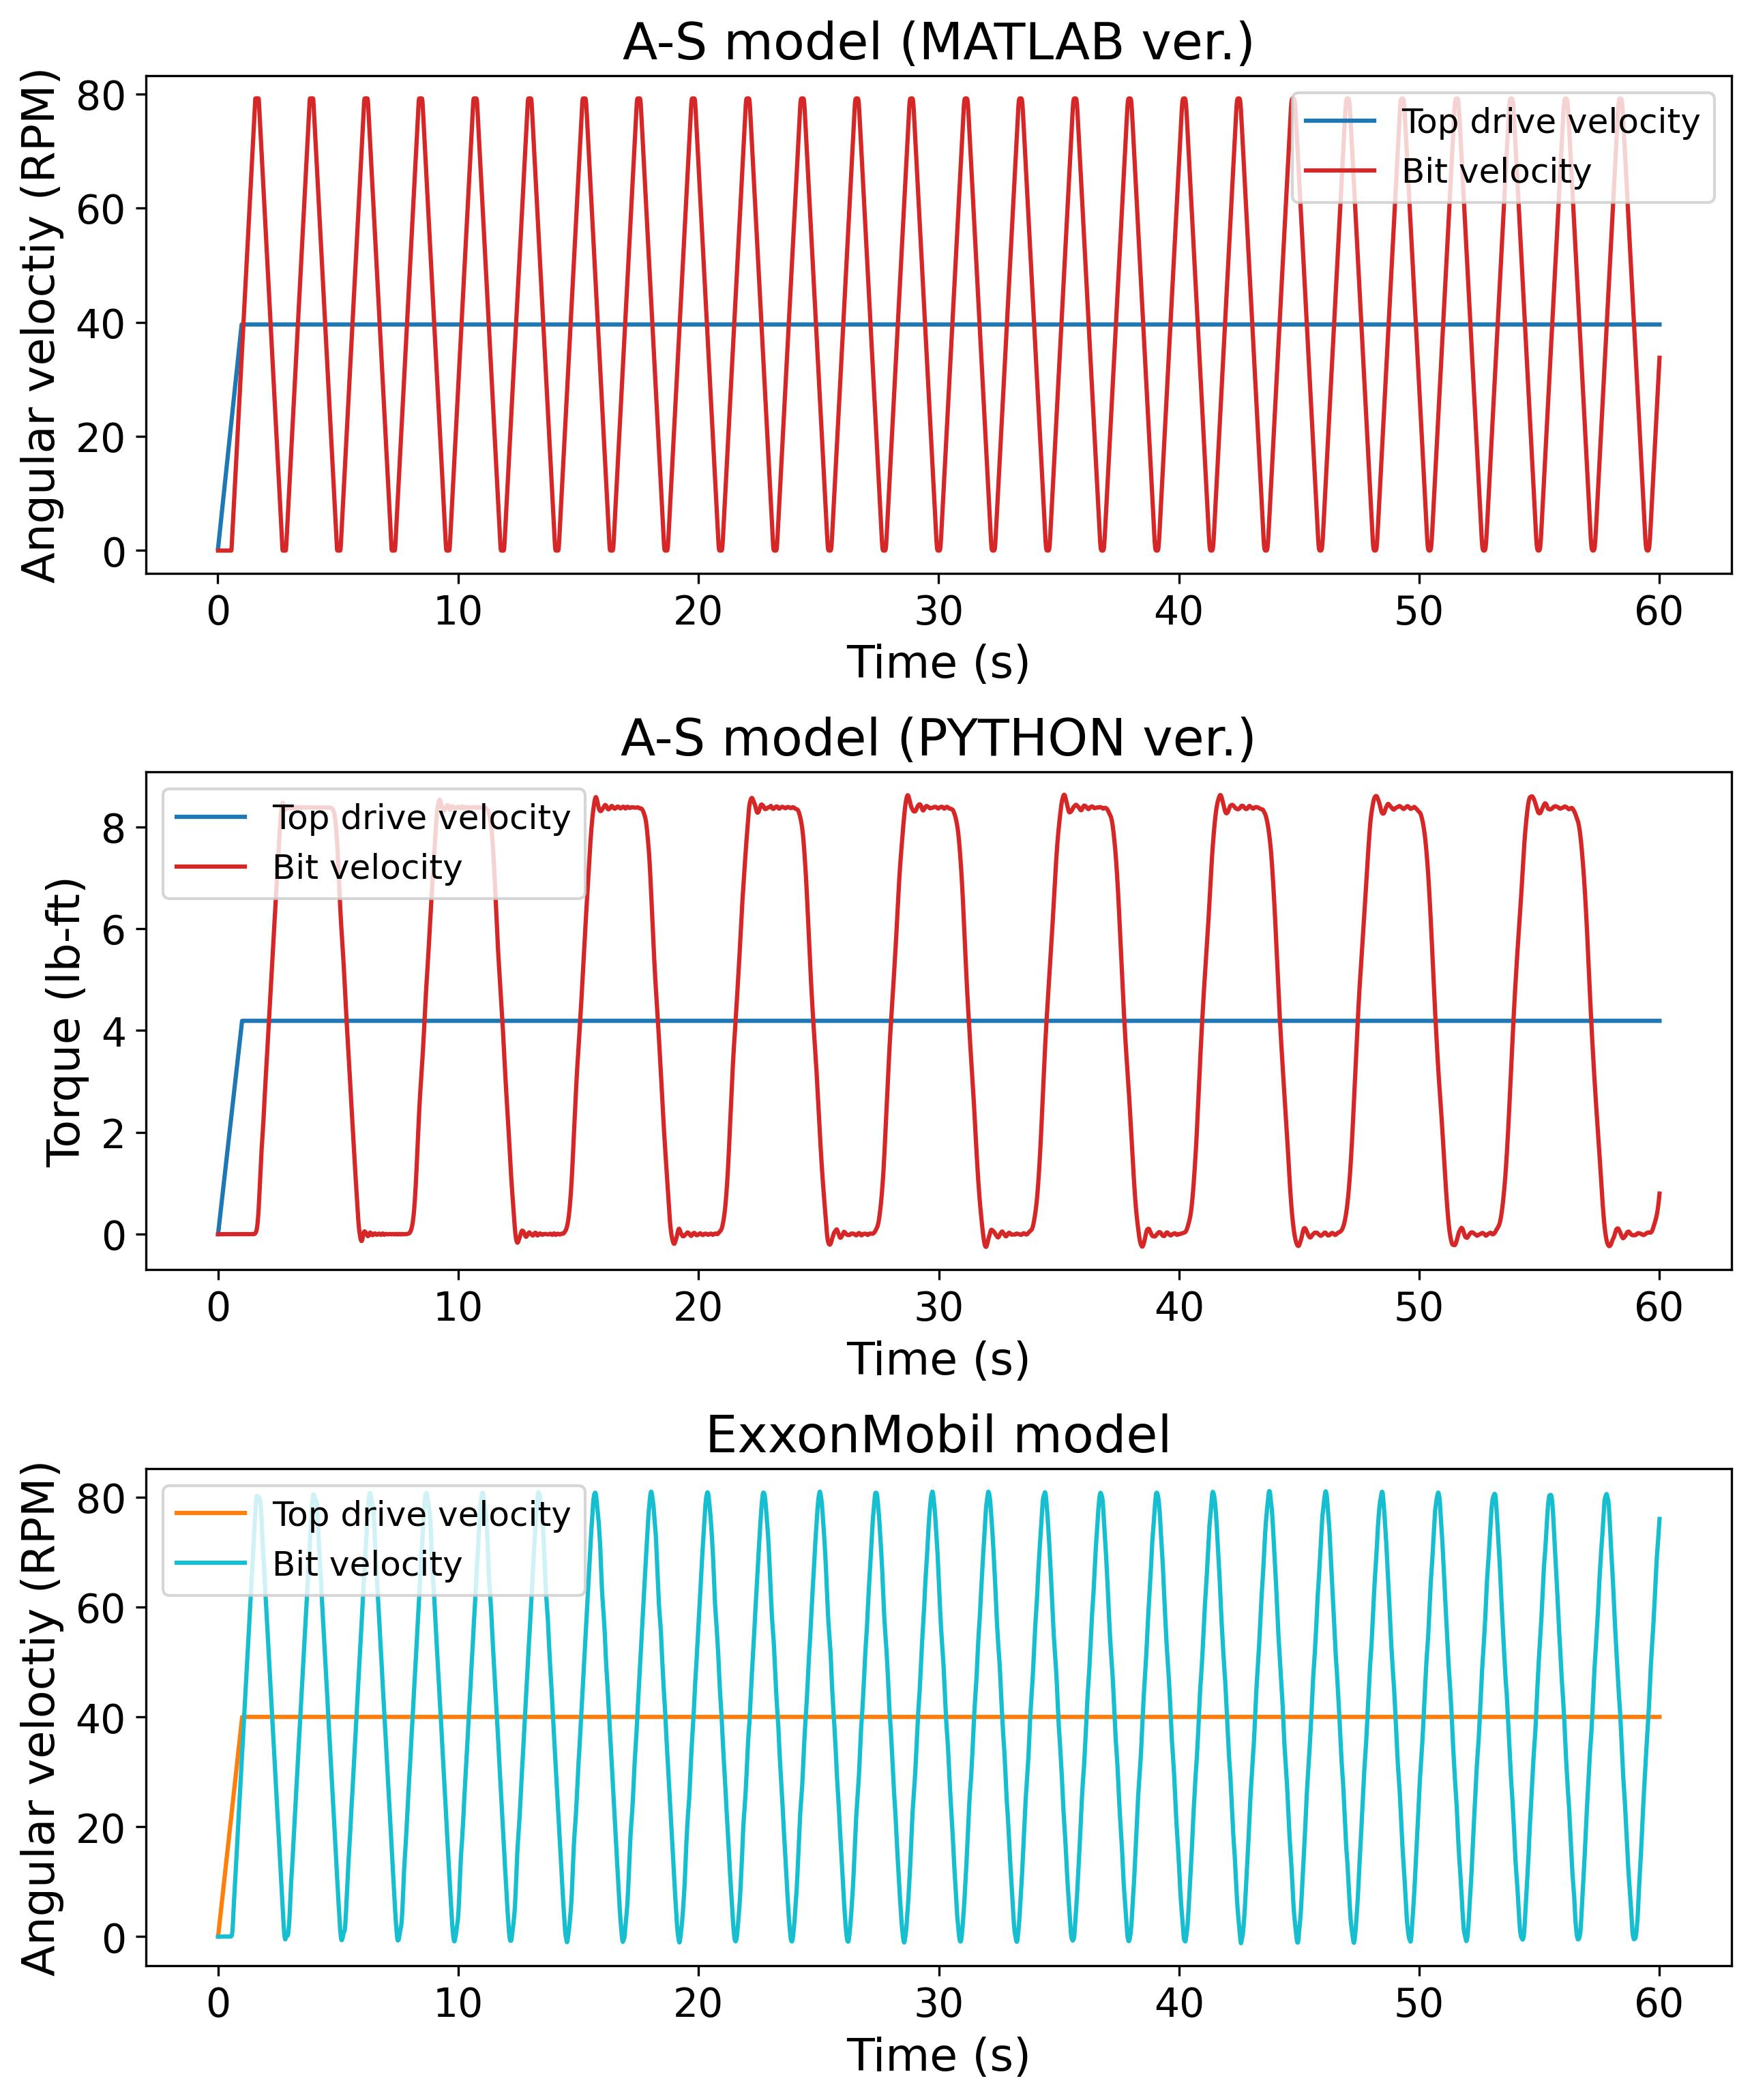
\includegraphics[height=4.5in]{version_comp}
  \caption[Comparison between different models for Test case 1]{Comparison of angular velocity of bit and top drive between A-S model Matlab, Python ver.\ and ExxonMobil model for Test Case 1.}\label{figure_Test1_comp_chASmodel}
\end{figure}

\newpage
\begin{figure}[!hbt]
  \centering
  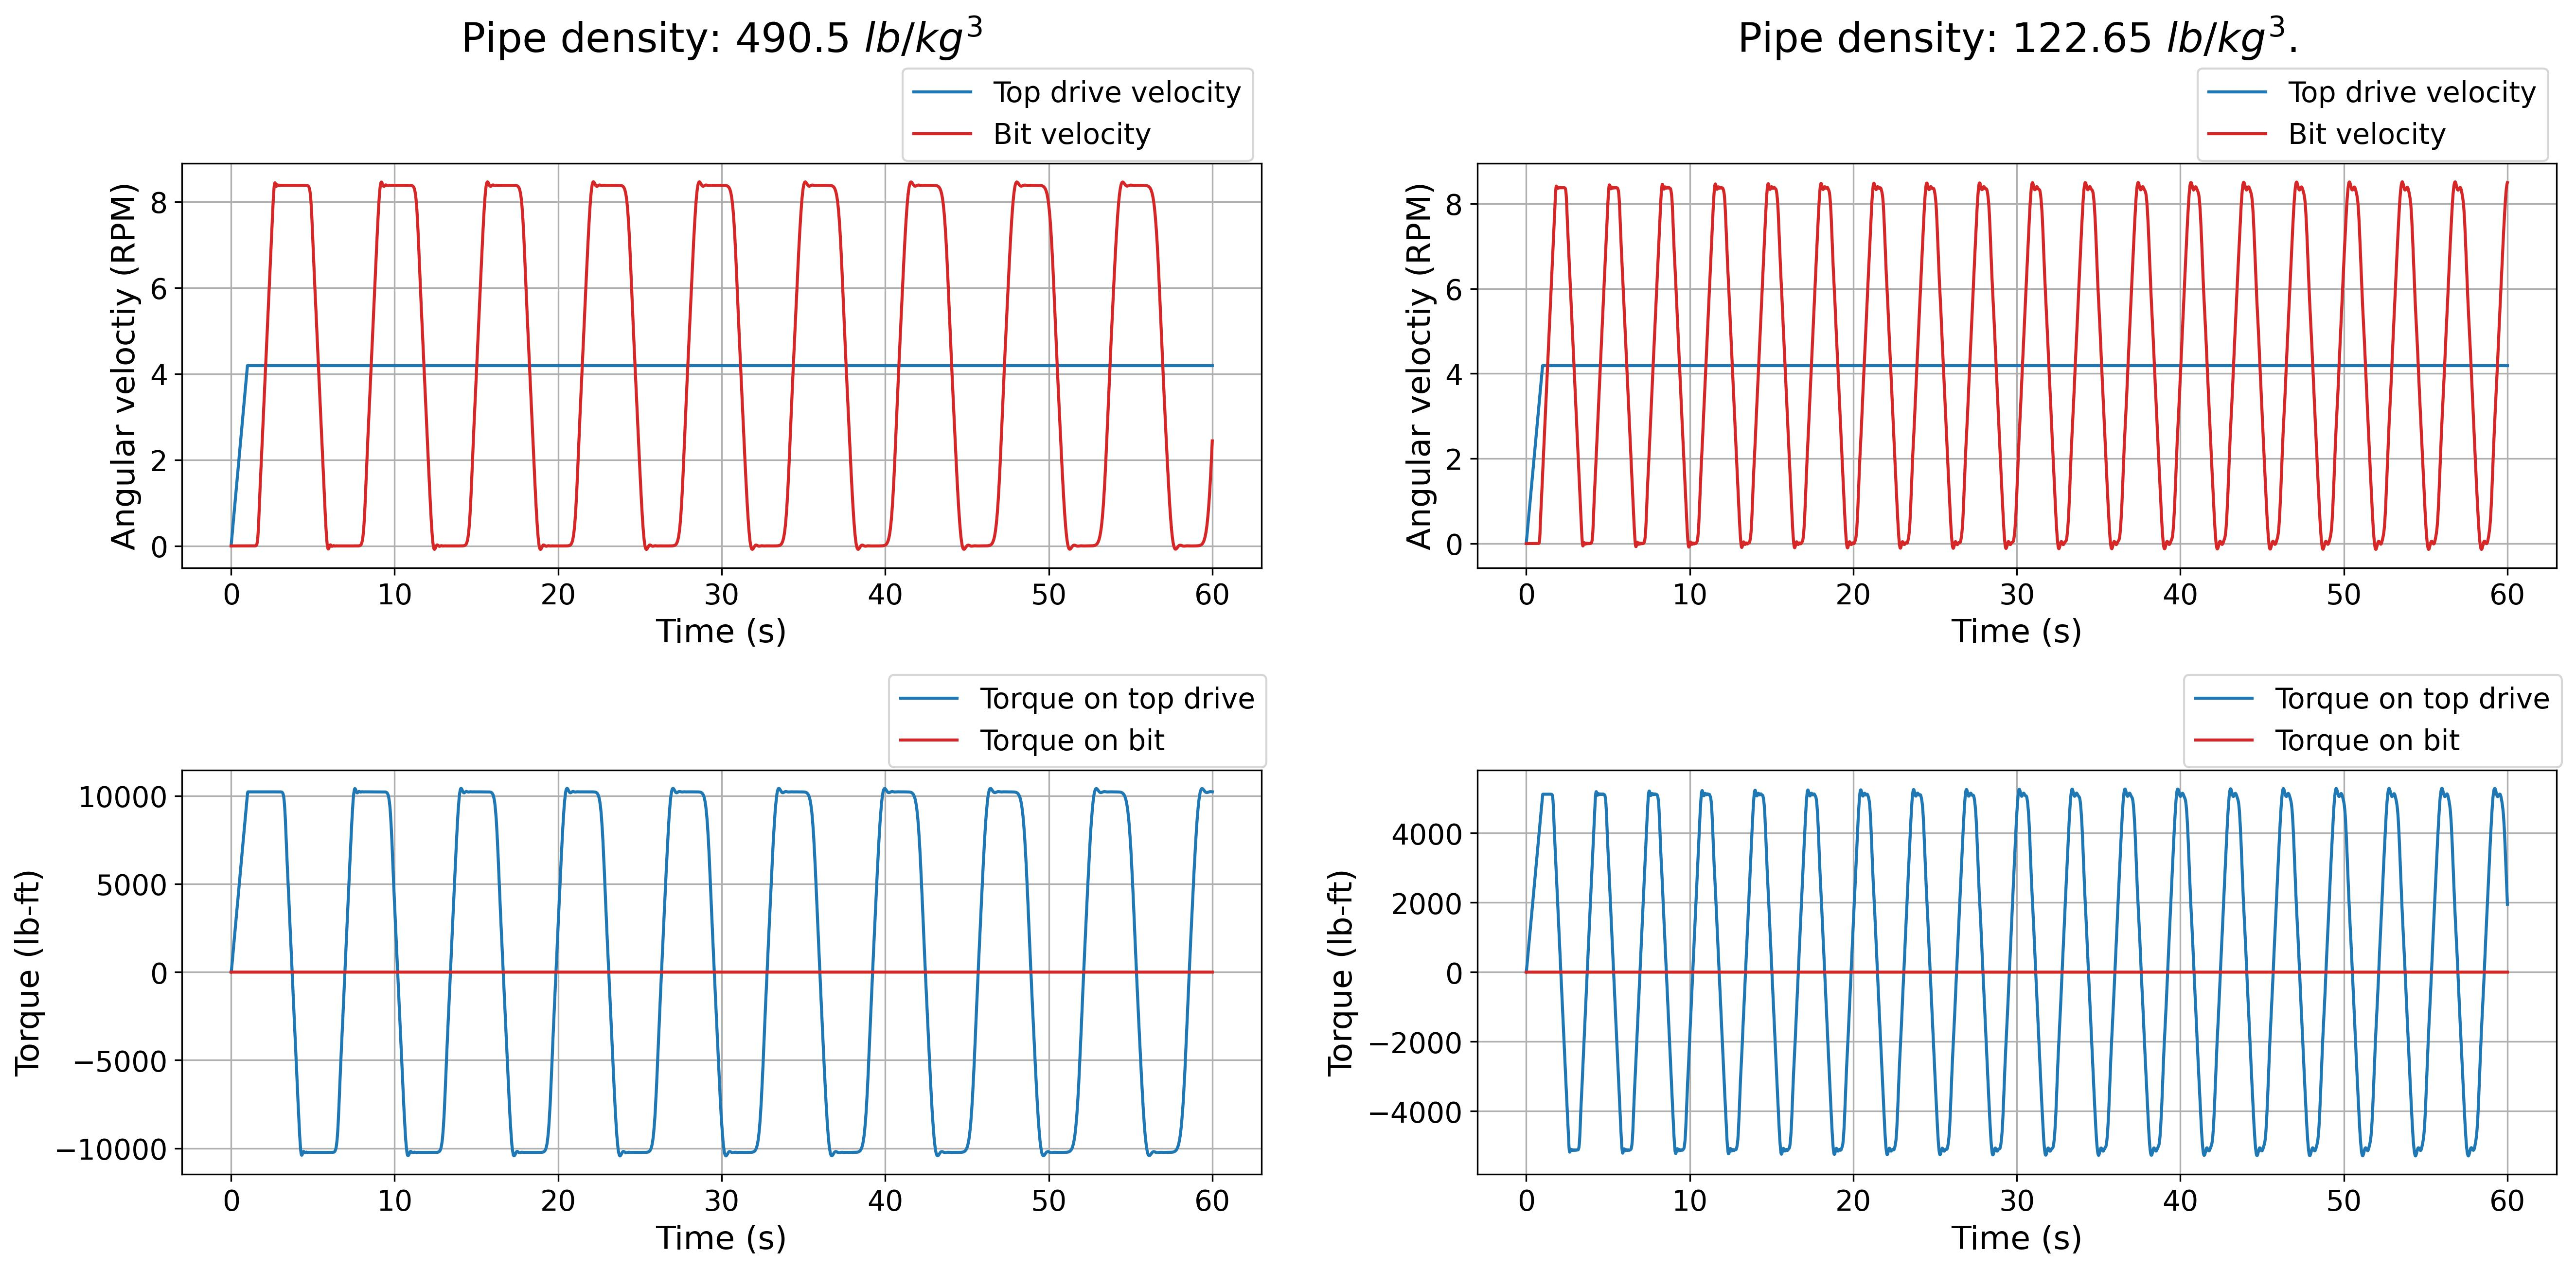
\includegraphics[width=6.5in]{density_comp}
  \caption[Effect of drill pipe density in Python ver.\ for Test Case 1]{Effect of drill pipe density to drill string vibration for A-S model, Python ver.\ for Test Case 1.  The first and second columns show the results with $\rho$ = 409.5 $lb/ft^3$ and  $\rho$ = 122.65 $lb/ft^3$, respectively.}\label{figure_Python_reducedDensity}
\end{figure}

 
